\section{Durchführung}
<<<<<<< HEAD:Fertig/V354/content/durchfuehrung.tex
\label{sec:Durchfuehrung}
||||||| merged common ancestors
<<<<<<< HEAD
\label{sec:Durchführung}
=======
\label{sec:durchfuehrung}
=======
\label{sec:durchfuehrung}
>>>>>>> update:V354/content/durchfuehrung.tex

\subsection{Zeitabhängigkeit der Amplitude einer gedämpften Schwingung}
Im ersten Teil wird die Zeitabhängigkeit der Amplitude einer gedämpften Schwingung untersucht. Im Anschluss kann 
daraus in der Auswertung ein Wert für den effektiven Dämpfungswiderstand ermittelt werden. 
Dafür wird mit einem Rechteckimpulsgenerator der Schwingkreis zu einer gedämpften Schwingung angeregt.
In der Schaltung wird dazu der kleine Festwiderstand verwendet.
<<<<<<< HEAD:Fertig/V354/content/durchfuehrung.tex
\begin{figure}
    \centering
    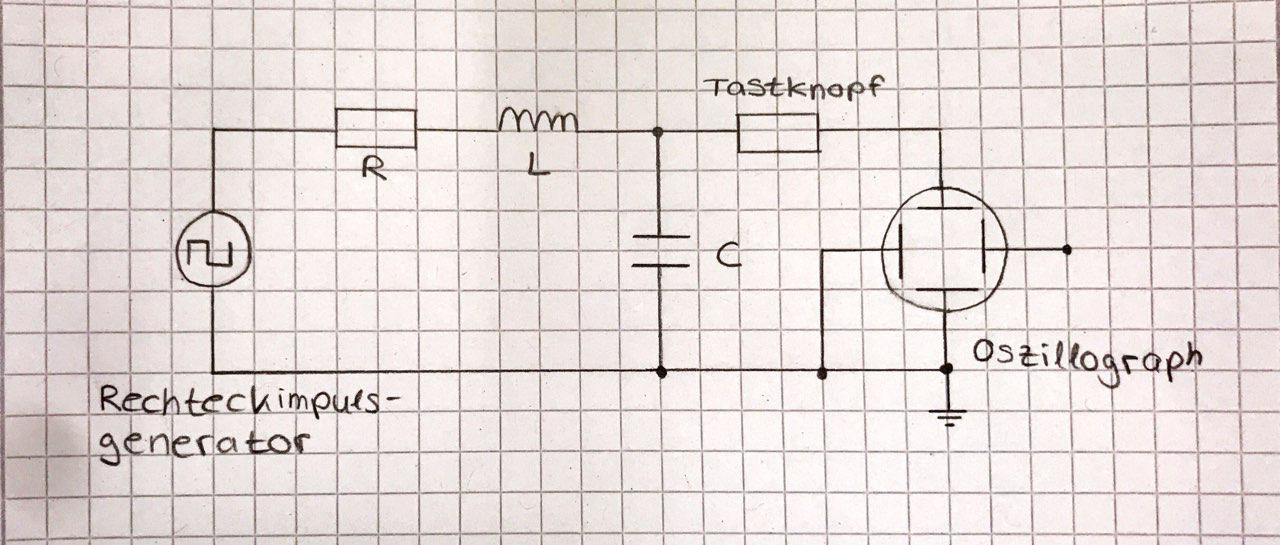
\includegraphics[width= 10cm, height= 7cm]{build/a.jpg}
    \caption{Schaltkreis zur Bestimmung der Zeitabhängigkeit der Amplitude.}
    \label{fig:a}
\end{figure}
||||||| merged common ancestors
%\begin{figure}
%    \centering
%    \includegraphics{}
%    \caption{Schaltkreis zur Bestimmung der Zeitabhängigkeit der Amplitude.}
%    \label{fig:a}
%\end{figure}
=======
>>>>>>> update:V354/content/durchfuehrung.tex

\subsection{Bestimmung des Dämpfungswiderstands}
Durch Variation des regelbaren Widerstands kann der Wert $R_{ap}$ ermittelt werden, bei dem der aperiodische
Grenzfall erreicht wird.
Der Widerstand wird am Anfang auf seinen Minimalwert eingestellt. Nach und nach wird der Widerstand dann erhöht. 
Sobald ein Kurvenbereich auftritt, in dem die Steigung des Graphen $\frac{dU_{C}}{dt}$ größer 0 ist, wurde 
$R_{ap}$ überschritten. Auf diese Weise lässt sich ablesen, wie groß der Dämpfungswiderstand $R_{ap}$
sein muss, um den aperiodischen Grenzfall zu erreichen.
<<<<<<< HEAD:Fertig/V354/content/durchfuehrung.tex
\begin{figure}
    \centering
    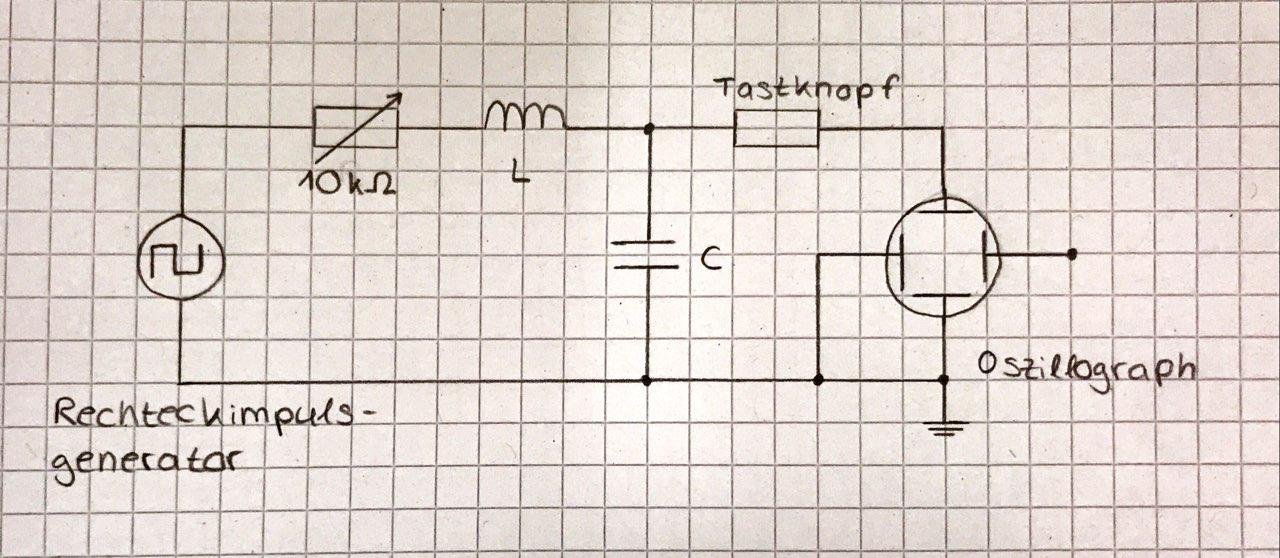
\includegraphics[width= 10cm, height= 7cm]{build/b.jpg}
    \caption{Schaltkreis zur Bestimmung des Dämpfungswiderstands beim aperiodischen Grenzfall.}
    \label{fig:b}
\end{figure}
||||||| merged common ancestors
%\begin{figure}
%    \centering
%    \includegraphics{}
%    \caption{Schaltkreis zur Bestimmung des Dämpfungswiderstands beim aperiodischen Grenzfall.}
%    \label{fig:b}
%\end{figure}
=======
>>>>>>> update:V354/content/durchfuehrung.tex

\subsection{Frequenzabhängigkeit der Kondensatorspannung}
\label{sec:c}
Die Kondesatorspannung und deren Frequenzabhängigkeit wird an einem Serienresonanzkreis gemessen. Hierfür wird eine 
Wechselspannung an den Schwingkreis angeschlossen. An einem Sinusspannungsgenerator wird die Frequenz eingestellt.
Die Kondensatorspannung wird mit einem Oszilloskop gemessen. Der Dämpfunswiderstand soll hierbei der 
größere der beiden Festwiderstände sein. %Auch der Dämpfungswiderstand des Sinusgenerators ist mit zu kalkulieren. NÖ
Insgesamt werden 30 Messwertpaare aufgenommen. Im Bereich von $\num{9}$ bis $\SI{29}{\kilo\hertz}$ und
im Bereich von $\num{39}$ bis $\SI{59}{\kilo\hertz}$ wird jeweils in $\SI{2}{\kilo\hertz}$ Schritten
gemessen. Im Bereich von $\num{29}$ bis $\SI{39}{\kilo\hertz}$ wird in $\SI{1}{\kilo\hertz}$ Schritten
gemessen.
<<<<<<< HEAD:Fertig/V354/content/durchfuehrung.tex
\begin{figure}
    \centering
    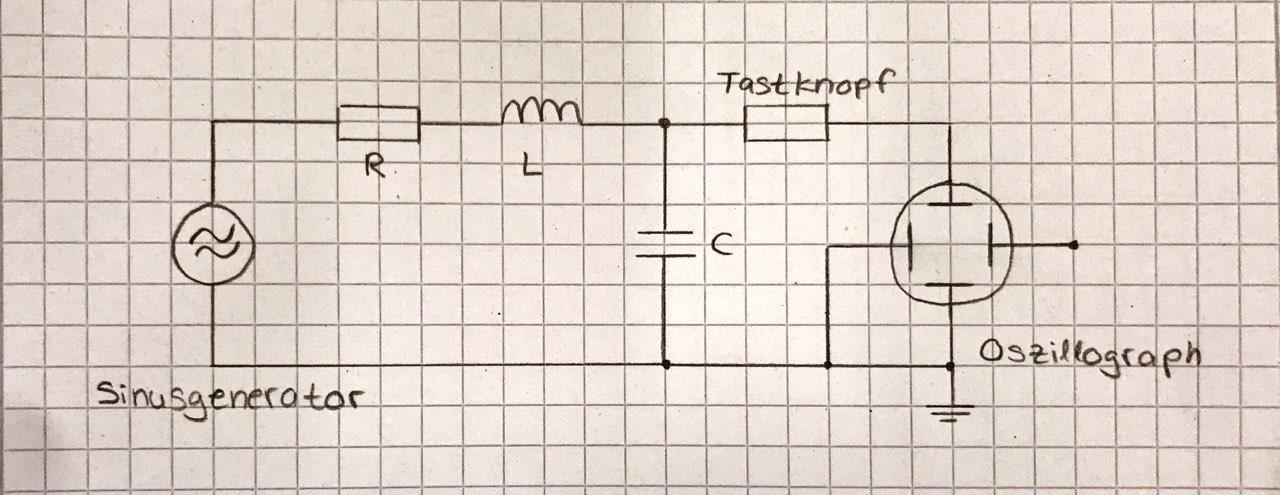
\includegraphics[width= 10cm, height= 7cm]{build/c.jpg}
    \caption{Schaltkreis zur Bestimmung der Frequenzabhängigkeit der Kondensatorspannung und der Phase.}
    \label{fig:c}
\end{figure}
||||||| merged common ancestors
%\begin{figure}
%    \centering
%    \includegraphics{}
%    \caption{Schaltkreis zur Bestimmung der Frequenzabhängigkeit der Kondensatorspannung und der Phase.}
%    \label{fig:c}
%\end{figure}
=======
>>>>>>> update:V354/content/durchfuehrung.tex

\subsection{Frequenzabhängigkeit der Phase}
Anschließend wird die Frequenzabhängigkeit der Phase zwischen Erreger- und Kondensatorspannung verglichen. Dafür 
wird der zeitliche Abstand der beiden Nulldurchgänge der Schwingungen gemessen. Die benötigte Periodendauer ergibt sich aus der eingestellten
<<<<<<< HEAD:Fertig/V354/content/durchfuehrung.tex
Frequenz. Die Messbereiche sind hier die selben wie in \ref{sec:c}.
Der Schaltkreis aus Abb. \ref{fig:c} wird auch für diese Messung verwendet.
||||||| merged common ancestors
Frequenz. Die Messbereiche sind hier die selben wie in \ref{sec:c}.
%Der Schaltkreis aus Abb. \ref{fig:c} wird auch für diese Messung verwendet.
>>>>>>> 252b602da14c14809158feb7356a846e65290dca
=======
Frequenz. Die Messbereiche sind hier die selben wie in \ref{sec:c}.
>>>>>>> update:V354/content/durchfuehrung.tex
